\begin{table}[!htb]
    \centering
    \caption{Impact of structural pruning with and without KALE on Accuracy at 100 across various datasets. }
    \tiny
    \scalebox{0.8}{
    \begin{tabular}{|l|l|l|l|l|l|l|}
    \hline
        Layers & KALE & NQ & TriviaQA & MSMARCO & SCIFACT & SQUAD \\ \hline
        12 & N/A & 85.84\% & 85.84\% & 88.77\% & 90.70\% & 77.16\% \\ \hline
        9 & N & 79.97\% & 79.97\% & 82.01\% & 71.07\% & 71.38\% \\ \hline
        9 & Y & 84.90\% & 84.90\% & 86.16\% & 84.87\% & 73.54\% \\ \hline
        6 & N & 68.20\% & 68.20\% & 72.68\% & 22.98\% & 59.97\% \\ \hline
        6 & Y & 83.68\% & 83.68\% & 84.68\% & 85.13\% & 69.87\% \\ \hline
        3 & N & 43.88\% & 43.88\% & 11.39\% & 40.80\% & 34.42\% \\ \hline
        3 & Y & 81.14\% & 81.14\% & 82.11\% & 82.57\% & 64.37\% \\ \hline
        2 & N & 46.90\% & 46.90\% & 31.46\% & 42.66\% & 37.01\% \\ \hline
        2 & Y & 81.94\% & 81.94\% & 81.96\% & 82.57\% & 63.72\% \\ \hline
        1 & N & 12.22\% & 12.22\% & 0.00\% & 3.17\% & 11.66\% \\ \hline
        1 & Y & 71.33\% & 71.33\% & 54.36\% & 66.83\% & 51.39\% \\ \hline
    \end{tabular}}
    \label{tab:kale-at-20}
\end{table}
While training asymmetric models can improve latency, it requires novel training regimes and experimentation, and existing workloads need to regenerate their entire index to take advantage of any inference speedups. Generation of the passage index can take longer than model training \cite{Karpukhin2020DensePR}, which makes regenerating a new index and retraining a model to meet changing latency requirements an inefficient experimentation pathway. \\Moreover, coupling asymmetry into training makes generating query encoder variants more difficult, as each encoder requires its own index and document encoder. \\
Motivated by this bottleneck, we introduce \textbf{K}ullback-Leibler \textbf{Al}lingment of \textbf{E}mbeddings (KALE), a simple method of improving bi-encoder latency by aligning the embeddings of compressed models. KALE is applied after model training and leverages large batch sizes to make compression \textbf{computationally inexpensive} and \textbf{independent of training}. A single V100 GPU KALE can produce a compressed query encoder in less than 5 minutes.  \\
First, a bi-encoder model trains with separate query and document encoders. When training is complete, the document encoder, $e_{document}$, is frozen, and using the query encoder, $e_{q}$, a structurally pruned copy, $e_{q'}$, is made. Then, using a sample of queries, the $e_{q'}$ model is fine-tuned to minimize the KL divergence of their query representations as shown in equation \ref{kale-eq:1}. \\
\begin{equation}\label{kale-eq:1} 
    \displaystyle D_{\text{KL}}(e_{q'} \parallel e_{q} )= \sum _{x\in {\mathcal {X}}}e_{q'}(x)\log \left({\frac {e_{q'}(x)}{e_{q}(x)}}\right).
\end{equation}
We explored the use of various distance functions such as cosine similarity, Manhattan distance, and the KL divergence but found little sensitivity in any metric besides KL divergence. We believe this is due to us freezing the document representations, and as a result, cosine distance allows the query embeddings to \textit{drift} more than probability distribution matching methods. To explore this further, we experiment with tuning the temperature for the KL divergence and add a loss scaling factor but find a temperature of one and a scaling factor of ten to be most optimal. \\
Additionally, we explored using a contrastive loss with random negative and hard negatives mined from the trained encoder but found no positive impact for either method. We leave further exploration of training objective improvement for future work.
\begin{figure*}
    \centering
    \begin{subfigure}[b]{0.35\textwidth}
   \begin{adjustbox}{width=\linewidth}
      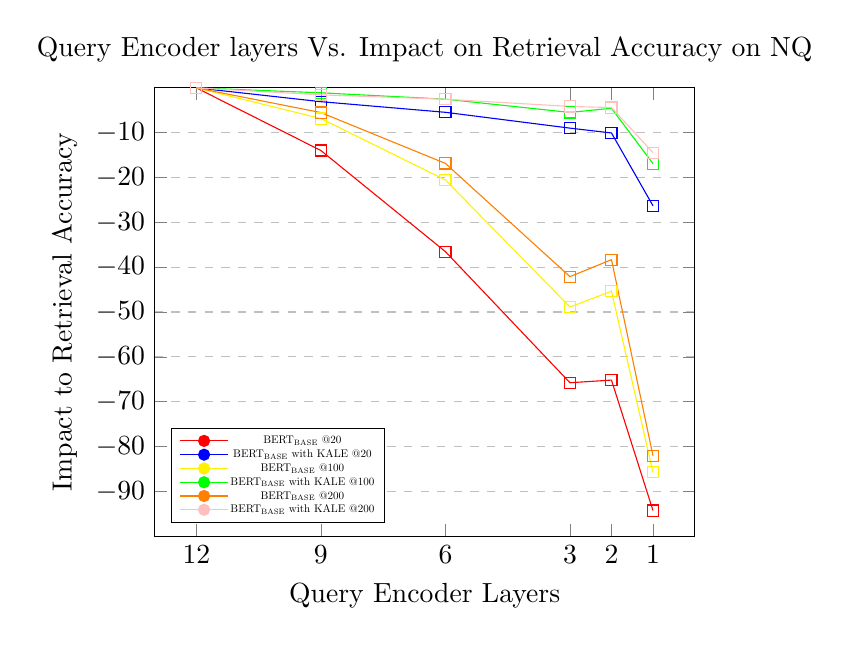
\begin{tikzpicture}
\begin{axis}[
    title={Query Encoder layers Vs. Impact on Retrieval Accuracy on NQ},
    xlabel={Query Encoder Layers},
    ylabel={Impact to Retrieval Accuracy},
    xmin=0, xmax=13,
    x dir=reverse,
    ymin=-100 , ymax=0,
    xtick={1,2,3,6,9,12},
    ytick={-10,-20,-30,-40, -50,-60,-70,-80,-90},
    legend pos=south west,
    ymajorgrids=true,
    grid style=dashed,
    legend style={nodes={scale=0.4, transform shape}}, 
    legend image post style={mark=*}
]
\addplot[
    color=red,
    mark=square,
    ]
    coordinates {
    (12, 0) (9, -13.97) (6,-36.53) (3,-65.77) (2, -65.18) (1, -94.28)
    };

\addplot[
    color=blue,
    mark=square,
    ]
    coordinates {
    (12, 0) (9, -3.08) (6, -5.45) (3,-8.98) (2,-10.06) (1, -26.30)

    };
\addplot[
    color=yellow,
    mark=square,
    ]
    coordinates {
    (12, 0) (9, -6.84) (6,-20.55) (3,-48.88) (2, -45.36) (1, -85.76)
    };

\addplot[
    color=green,
    mark=square,
    ]
    coordinates {
    (12, 0) (9, -1.10) (6, -2.52) (3,-5.48) (2,-4.54) (1, -16.90)

    };
\addplot[
    color=orange,
    mark=square,
    ]
    coordinates {
    (12, 0) (9, -5.51) (6,-16.85) (3,-42.11) (2, -38.32) (1, -82.05)
    };

\addplot[
    color=pink,
    mark=square,
    ]
    coordinates {
    (12, 0) (9, -1.56) (6, -2.53) (3,-4.14) (2,-4.39) (1, -14.44)

    };
\legend{BERT\textsubscript{BASE} @20, BERT\textsubscript{BASE} with KALE @20,BERT\textsubscript{BASE} @100, BERT\textsubscript{BASE} with KALE @100,BERT\textsubscript{BASE} @200, BERT\textsubscript{BASE} with KALE @200}
 \end{axis}
\end{tikzpicture}
 \end{adjustbox} 
\end{subfigure} 
    \begin{subfigure}[b]{0.382\textwidth}
   \begin{adjustbox}{width=\linewidth} 
      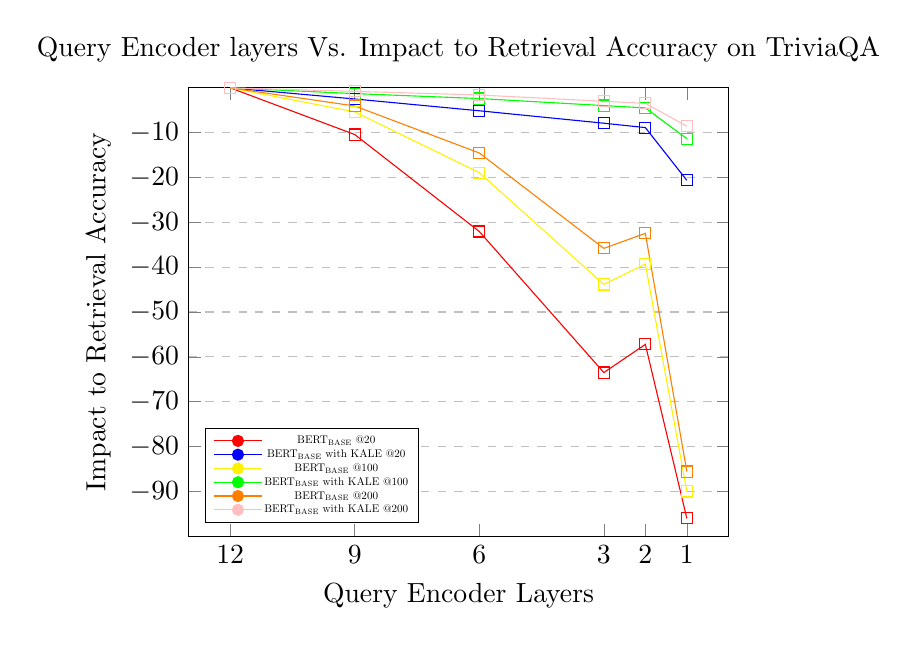
\begin{tikzpicture}
        \begin{axis}[
            title={Query Encoder layers Vs. Impact to Retrieval Accuracy on TriviaQA},
            xlabel={Query Encoder Layers},
            ylabel={Impact to Retrieval Accuracy},
            xmin=0, xmax=13,
            x dir=reverse,
            ymin=-100 , ymax=0,
            xtick={1,2,3,6,9,12},
            ytick={-10,-20,-30,-40, -50,-60,-70,-80,-90},
            legend pos=south west,
            ymajorgrids=true,
            grid style=dashed,
            legend style={nodes={scale=0.4, transform shape}}, 
            legend image post style={mark=*}
        ]
        \addplot[
            color=red,
            mark=square,
            ]
            coordinates {
            (12, 0) (9, -10.41) (6,-32.04) (3,-63.5) (2, -57.22) (1, -96.03)
            };
        
        \addplot[
            color=blue,
            mark=square,
            ]
            coordinates {
            (12, 0) (9, -2.48) (6, -5.11) (3,-7.88) (2,-8.86) (1, -20.63)
        
            };
        \addplot[
            color=yellow,
            mark=square,
            ]
            coordinates {
            (12, 0) (9, -5.35) (6,-18.91) (3,-43.84) (2, -39.29) (1, -90.02)
            };
        
        \addplot[
            color=green,
            mark=square,
            ]
            coordinates {
            (12, 0) (9, -1.28) (6,-2.38) (3,-3.95) (2, -4.47) (1, -11.33)
            };
        
        \addplot[
            color=orange,
            mark=square,
            ]
            coordinates {
            (12, 0) (9, -4.04) (6, -14.52) (3,-35.8) (2,-32.45) (1, -85.58)
        
            };
        \addplot[
            color=pink,
            mark=square,
            ]
            coordinates {
            (12, 0) (9, -0.78) (6,-1.59) (3,-2.99) (2, -3.45) (1, -8.54)
            };
        \legend{BERT\textsubscript{BASE} @20, BERT\textsubscript{BASE} with KALE @20,BERT\textsubscript{BASE} @100, BERT\textsubscript{BASE} with KALE @100,BERT\textsubscript{BASE} @200, BERT\textsubscript{BASE} with KALE @200}
         \end{axis}
        \end{tikzpicture}
         \end{adjustbox}       
    \end{subfigure}
    \\
    \begin{subfigure}[b]{0.4\textwidth}
       \begin{adjustbox}{width=\linewidth} % rescale box
          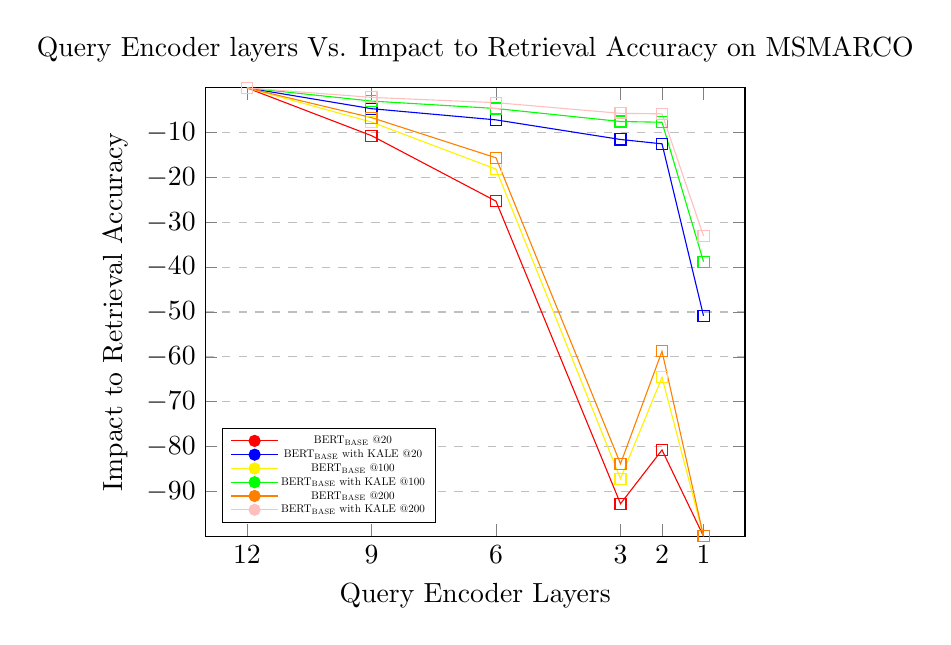
\begin{tikzpicture}
            \begin{axis}[
                title={Query Encoder layers Vs. Impact to Retrieval Accuracy on MSMARCO},
                xlabel={Query Encoder Layers},
                ylabel={Impact to Retrieval Accuracy},
                xmin=0, xmax=13,
                x dir=reverse,
                ymin=-100 , ymax=0,
                xtick={1,2,3,6,9,12},
                ytick={-10,-20,-30,-40, -50,-60,-70,-80,-90},
                legend pos=south west,
                ymajorgrids=true,
                grid style=dashed,
                legend style={nodes={scale=0.4, transform shape}}, 
                legend image post style={mark=*}
            ]
            \addplot[
                color=red,
                mark=square,
                ]
                coordinates {
                (12, 0) (9, -10.65) (6,-25.27) (3,-92.76) (2, -80.77) (1, -100)
                };
            
            \addplot[
                color=blue,
                mark=square,
                ]
                coordinates {
                (12, 0) (9, -4.64) (6, -7.14) (3,-11.51) (2,-12.48) (1, -50.84)
            
                };
            \addplot[
                color=yellow,
                mark=square,
                ]
                coordinates {
                (12, 0) (9, -7.62) (6,-18.12) (3,-87.17) (2, -64.56) (1, -100)
                };
            
            \addplot[
                color=green,
                mark=square,
                ]
                coordinates {
                (12, 0) (9, -2.94) (6, -4.6) (3,-7.5) (2,-7.67) (1, -38.77)
            
                };
            \addplot[
                color=orange,
                mark=square,
                ]
                coordinates {
                (12, 0) (9, -6.63) (6,-15.6) (3,-83.85) (2, -58.75) (1, -100)
                };
            
            \addplot[
                color=pink,
                mark=square,
                ]
                coordinates {
                (12, 0) (9, -2.12) (6, -3.3) (3,-5.68) (2,-5.79) (1, -33.05)
            
                };
            \legend{BERT\textsubscript{BASE} @20, BERT\textsubscript{BASE} with KALE @20,BERT\textsubscript{BASE} @100, BERT\textsubscript{BASE} with KALE @100,BERT\textsubscript{BASE} @200, BERT\textsubscript{BASE} with KALE @200}
             \end{axis}
            \end{tikzpicture}
        \end{adjustbox}       
    \end{subfigure} \\ 
    \begin{subfigure}[b]{0.38\textwidth}
       \begin{adjustbox}{width=\linewidth} % rescale box
          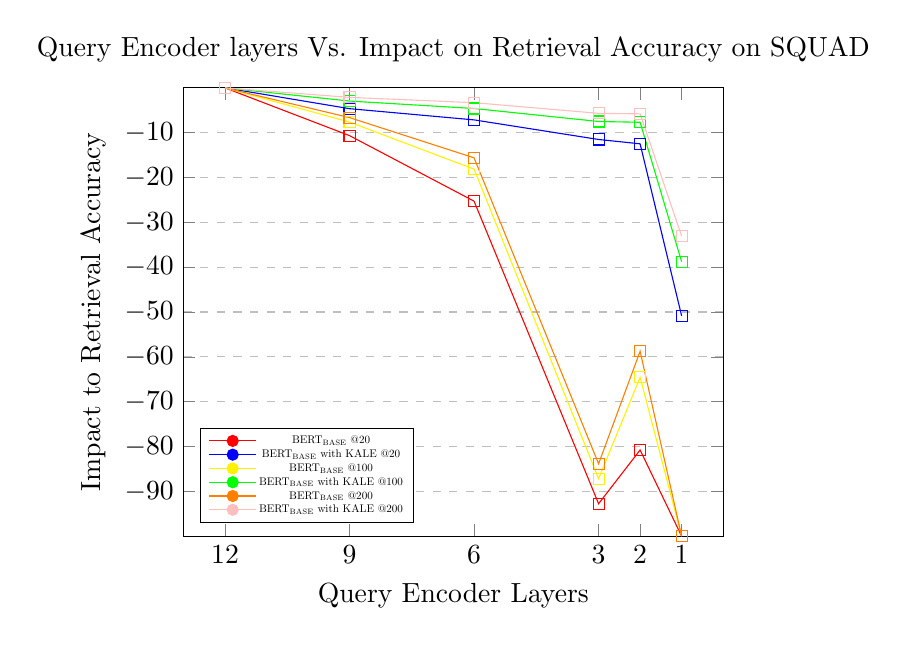
\begin{tikzpicture}
            \begin{axis}[
                title={Query Encoder layers Vs. Impact on Retrieval Accuracy on SQUAD},
                xlabel={Query Encoder Layers},
                ylabel={Impact to Retrieval Accuracy},
                xmin=0, xmax=13,
                x dir=reverse,
                ymin=-100 , ymax=0,
                xtick={1,2,3,6,9,12},
                ytick={-10,-20,-30,-40, -50,-60,-70,-80,-90},
                legend pos=south west,
                ymajorgrids=true,
                grid style=dashed,
                legend style={nodes={scale=0.4, transform shape}}, 
                legend image post style={mark=*}
            ]
            \addplot[
                color=red,
                mark=square,
                ]
                coordinates {
                (12, 0) (9, -10.65) (6,-25.27) (3,-92.76) (2, -80.77) (1, -100)
                };
            
            \addplot[
                color=blue,
                mark=square,
                ]
                coordinates {
                (12, 0) (9, -4.64) (6, -7.14) (3,-11.51) (2,-12.48) (1, -50.84)
            
                };
            \addplot[
                color=yellow,
                mark=square,
                ]
                coordinates {
                (12, 0) (9, -7.62) (6,-18.12) (3,-87.17) (2, -64.56) (1, -100)
                };
            
            \addplot[
                color=green,
                mark=square,
                ]
                coordinates {
                (12, 0) (9, -2.94) (6, -4.6) (3,-7.5) (2,-7.67) (1, -38.77)
            
                };
            \addplot[
                color=orange,
                mark=square,
                ]
                coordinates {
                (12, 0) (9, -6.63) (6,-15.6) (3,-83.85) (2, -58.75) (1, -100)
                };
            
            \addplot[
                color=pink,
                mark=square,
                ]
                coordinates {
                (12, 0) (9, -2.12) (6, -3.3) (3,-5.68) (2,-5.79) (1, -33.05)
            
                };
            \legend{BERT\textsubscript{BASE} @20, BERT\textsubscript{BASE} with KALE @20,BERT\textsubscript{BASE} @100, BERT\textsubscript{BASE} with KALE @100,BERT\textsubscript{BASE} @200, BERT\textsubscript{BASE} with KALE @200}
             \end{axis}
            \end{tikzpicture}
        \end{adjustbox}
    \end{subfigure} 
    \begin{subfigure}[b]{0.4\textwidth}
       \begin{adjustbox}{width=\linewidth} % rescale box
          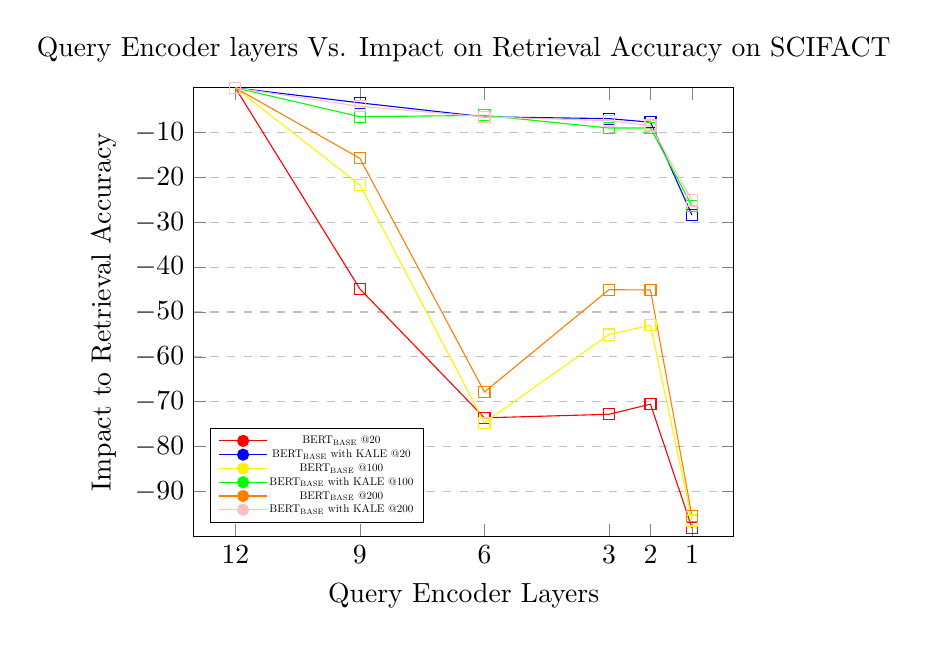
\begin{tikzpicture}
            \begin{axis}[
                title={Query Encoder layers Vs. Impact on Retrieval Accuracy on SCIFACT},
                xlabel={Query Encoder Layers},
                ylabel={Impact to Retrieval Accuracy},
                xmin=0, xmax=13,
                x dir=reverse,
                ymin=-100 , ymax=0,
                xtick={1,2,3,6,9,12},
                ytick={-10,-20,-30,-40, -50,-60,-70,-80,-90},
                legend pos=south west,
                ymajorgrids=true,
                grid style=dashed,
                legend style={nodes={scale=0.4, transform shape}}, 
                legend image post style={mark=*}
            ]
            \addplot[
                color=red,
                mark=square,
                ]
                coordinates {
                (12, 0) (9, -44.85) (6,-73.60) (3,-72.81) (2, -70.55) (1, -98.18)
                };
            
            \addplot[
                color=blue,
                mark=square,
                ]
                coordinates {
                (12, 0) (9, -3.34) (6,-6.45) (3,-6.86) (2, -7.66) (1, -28.38)
                };
            \addplot[
                color=yellow,
                mark=square,
                ]
                coordinates {
                (12, 0) (9, -21.64) (6,-74.66) (3,-55.02) (2, -52.95) (1, -96.50)
                };
            
            \addplot[
                color=green,
                mark=square,
                ]
                coordinates {
                (12, 0) (9, -6.43) (6,-6.14) (3,-8.96) (2, -8.96) (1, -26.32)
                };
            \addplot[
                color=orange,
                mark=square,
                ]
                coordinates {
                (12, 0) (9, -15.72) (6,-67.83) (3,-45.01) (2, -45.09) (1, -95.49)
                };
            
            \addplot[
                color=pink,
                mark=square,
                ]
                coordinates {
                (12, 0) (9, -4.13) (6,-6.47) (3,-7.33) (2, -8.39) (1, -25.11)
                };
            \legend{BERT\textsubscript{BASE} @20, BERT\textsubscript{BASE} with KALE @20,BERT\textsubscript{BASE} @100, BERT\textsubscript{BASE} with KALE @100,BERT\textsubscript{BASE} @200, BERT\textsubscript{BASE} with KALE @200}
             \end{axis}
            \end{tikzpicture}
        \end{adjustbox}
    \end{subfigure}
    \caption{Impact of structural pruning with and without KALE on the NQ, MSMARCO, TriviaQA, SciFACT, and SQuAD Passage Retrieval dataset with the recall set sizes of 20,100, and 200. Across datasets, we see a consistent trend where KALE is effective but most effective when the network is heavily pruned and recall set sizes are small. When the model is pruned to 2 or 1 layer with a recall set size of 20, the difference between using KALE or not can be up to 10 times the loss in recall accuracy}
    \label{fig:kale-not}
\end{figure*}
\subsection{Experimental Results}
We evaluate the effectiveness of KALE by taking uncompressed BERT\textsubscript{BASE} models and pruning them with and without KALE on a variety of well-established passage retrieval benchmarks. First, models are trained, and indexes are generated using un-optimized BERT\textsubscript{BASE} models. Next, the document encoders are frozen, and the query encoders are structurally pruned to have 9,6,3,2 or 1 transformer layer. Finally, query encoders are aligned using KALE, and we compare the performance of compressed models by comparing the impact on retrieval accuracy at 20,100, and 200. \\
To aid reproducibility, each model is trained using the Tevatron \cite{Gao2022TevatronAE} \footnote{https://github.com/texttron/tevatron} library, which makes use of hugginface's transformers to provide a simple interface for exploring neural ranking models. Our experiments focus on the plain BERT\textsubscript{BASE}-uncased 12-layer transformer model. While never more capable models exist, the unaltered BERT model is widely used in production workloads, which our experiments seek to emulate. \\
Our work aims not to produce the highest possible retrieval accuracy for a dense encoder. Instead, our goal is to find the role of asymmetry in bi-encoder models. As a result, we leverage the well-established parameters in all of our experiments without using an advanced methodology like contrastive or curriculum learning. \\
There are fewer parameters for using KALE, and we deliberately do not optimize on anything but the loss between $e_{q}$ and $e_{q'}$. In general, higher degrees of pruning require longer training with smaller batches. \\ 
\textbf{Datasets} We use a wide variety of standard dense retrieval benchmarks, including MSMARCO V1.1 \footnote{https://huggingface.co/datasets/Tevatron/msmarco-passage} \cite{Campos2016MSMA}, NQ Passage Ranking \footnote{https://huggingface.co/datasets/Tevatron/wikipedia-nq} \cite{Kwiatkowski2019NaturalQA}, SciFact Passage Ranking \footnote{https://huggingface.co/datasets/Tevatron/scifact} \cite{Wadden2020FactOF}, TriviaQA passage Ranking \footnote{https://huggingface.co/datasets/Tevatron/wikipedia-trivia} \cite{Joshi2017TriviaQAAL}, and SQUAD Passage Ranking \footnote{https://huggingface.co/datasets/Tevatron/wikipedia-squad} \cite{Rajpurkar2016SQuAD10}. \\
For each dataset, we evaluate performance by measuring the recall accuracy with retrieval depths of 20,100, and 200. Additionally, for the MSMARCO dataset, we also report MRR@10; for Scifact, we also report NDCG @10 and RR@10. \\
\textbf{Computational Experiments}
Our experimentation on fine-tuning our compressed models uses a 16 GB V100 GPU. Experiments in bi-encoder model training leverage 1 V100 for the MSMARCO and 4 for each other experiment. Due to the vast number of models and datasets we train on, each experiment happens with the same fixed seed.  
